\chapter{Implementation and Evaluation}

\section{Implementation}

We first modified the Followup tool so that it can check Phantom classes. This is helpful in for benchmarks in Dacapo \cite{TamiFlex}. Also, we have added an argument number option, which means if we are finding out the followup methods for a certain function then we will visit the object corresponding to that argument. For example, If we want to visit the followup methods on the receiver object then we will mention it as "0" and all the other arguments will start from 1,2,3 etc.

The Followup tool was extended for handling pattern matching and generation of optimized code. These modifications enable the tool to more accurately and efficiently identify and optimize Java programs with expensive collection class functions.

We used this modified version of the followup tool for the implementation of CCAP tool. As discussed above we first wrote some rules into the rules file and gave it to CCAP-Parser. It parses all the rules and builds a syntax tree for verification. With the help of the syntax tree we extracted required data for CCAP-Map using Visitors generated by JTB.

\section{microbenchmarks}

we created 10 micro benchmarks for the evaluation of the CCAP tool. They were designed to test the effectiveness of the tool in identifying and optimizing specific patterns in code. These patterns included addAll followed by toString, retainAll followed by isEmpty, addAll followed by contains, and reverse followed by toString for ArrayLists, LinkedLists, HashSets, and TreeSets.

By creating these benchmarks, we were able to test the tool's ability to identify and optimize these specific patterns in different types of collections. This allowed to evaluate the tool's effectiveness in improving the performance of code that contains these patterns.

Using these benchmarks, we were able to perform initial testing of the tool and identify any potential issues or limitations. we will then use this information to refine and improve the tool's optimization strategies, making it more effective in identifying and optimizing patterns in real-world code.


\section{Evaluation}
As mentioned we have run this tool for above mentioned rules and run it on all micro benchmarks. The benchmarks were run with input such that the collection (either lists or sets) has 100,000 elements and the expensive function followed by cheaper function pattern involved for 50 times. The results of the evaluation are summarized in Fig 4.1.

\begin{tabular}{ |p{3cm}|p{4cm}|p{4cm}|p{3cm}|  }
\hline
\multicolumn{4}{|c|}{MicroBenchmark Evaluation} \\
\hline
Benchmark Name & Original Execution time (in msec) & Execution time after modification (in msec) & Improvement \\
\hline
SetRetainAll (HashSet) &517.3829 & 56.7131 & 9.12 times \\
SetRetainAll (TreeSet) &688.456549 & 80.882575 & 8.51 times \\
reverseString &303.0512 & 283.6689 & 1.07 times \\
addAllContains &35.4208 & 14.8522 & 2.38 times \\
addAllString    &1002.7952 & 847.1052 & 1.18 times \\
\hline
\end{tabular}

\begin{figure} [h]
    \centering
    %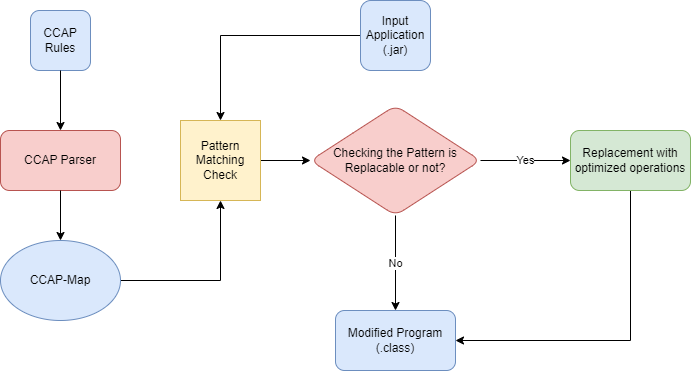
\includegraphics[width = \textwidth]{images/CCAP_tool.png}
    \caption{Microbenchmark Evaluation}
    \label{fig:my_label}
\end{figure}

After running the tool on these benchmarks, it was concluded that for larger numbers of elements in each collection, the tool worked well in optimizing the code and reducing the execution time. However, we also ran the code for smaller inputs. we found that, for smaller numbers of elements, some patterns such as addAllContains took more time than the original code. We believe that this unexpected behaviour is due to cache related issues which arises because of larger method bodies.

\begin{tabular}{ |p{3cm}|p{4cm}|p{4cm}|p{3cm}|  }
\hline
\multicolumn{4}{|c|}{MicroBenchmark Evaluation} \\
\hline
Benchmark Name & Original Execution time (in msec) & Execution time after modification (in msec) & Improvement \\
\hline
SetRetainAll (HashSet) &517.3829 & 56.7131 & 9.12 times \\
SetRetainAll (TreeSet) &688.456549 & 80.882575 & 8.51 times \\
reverseString &303.0512 & 283.6689 & 1.07 times \\
addAllContains &35.4208 & 14.8522 & 2.38 times \\
addAllString    &1002.7952 & 847.1052 & 1.18 times \\
\hline
\end{tabular}